% =====================================================================
%  Draft 2 Research Paper of This Project (21 Oct 2026)
%  E.C.H.O  (Efficient Contextualized History Orchestrator)
%
%  Built on the official IEEE Conference Template (IEEEtran, conference
%  mode, two columns). Upload this file as main.tex to Overleaf and it
%  compiles with pdfLaTeX without any other files (both figures are TikZ).
%
%  Draft 2 notes for the team:
%   * The paper describes the FINAL system as designed and decided on
%     2026-10-21 (decision ids A1..A43 in docs/review/ste_open_items.md),
%     not only the current build. Build runs Thu 22 to Sun 25 Oct 2026.
%     Claims beyond the current build (must be finished before submission):
%       - agentic retrieval loop: search_memories tool, up to 5 rounds,
%         usually 2 / max 6 LLM calls (A26); chat answers with memory pills
%         and a moment strip (A27); streamed progress over SSE (A28)
%       - local PostgreSQL + local Redis, schema opened (A31); visit table
%         for Chrome/YouTube with dwell per visit (A1.1, A1.1b); stored
%         tsvector + GIN index over the full text (A24.3)
%       - attachment text extracted at ingestion, incl. XLSX, PPTX, EML and
%         Tesseract OCR (A4, A22); query matched passages only (A23, A24.2)
%       - Gmail incremental polling with history.list, Spam/Trash skipped
%         (A5, A38); hidden preview text dropped, body parts joined (A6);
%         signature removal deleted (A12); inline replies kept (A14.2)
%       - Chrome: headings from the extension (A13), 38 word sensitive list
%         with whole token matching, secret query keys stripped, stricter
%         form check (A7), 7 app domains + public sections, rules served by
%         GET /chrome/rules (A9), Gmail web skipped (A9.1), app page minimum
%         on the server (A8.2), link clicks no longer count (A39 part 2)
%       - A39 timings (scroll 15 %, Shorts 10 s, completion 10 % with 5 s
%         floor, KNN from 5 items); YouTube 5 s revisit check (A34)
%       - Stage 3 richer seeds + seed threshold (A18), balanced recompute
%         (A20), recompute at worker start (A36), Stage 4 via Decisions API
%         on OpenAI (A21), curated domain map growth (A17)
%       - effort score: median for unread mail (A29); KNN only suggestion
%         threshold (A32); retention setting (A37); popup pause toggle (A33)
%       - automatic retry of failed enrichment items (carried over from
%         Draft 1; NOT scheduled by any decision, today manual via
%         ENP_RETRY_FAILED)
%   * Still open on 2026-10-21: A16 (embedding token budget), A40
%     (embedding model, \embmodel below), A42 (auto accept), A43 (user
%     groups under system groups), A11 outcome (transcripts, decided Thu).
%   * No measured results. Every number still to be measured is a visible
%     \tbd{...} placeholder. Search the PDF for "TBD".
%   * Style: plain wording, no hyphens or dashes in prose, US spelling.
% =====================================================================
\documentclass[conference]{IEEEtran}
\IEEEoverridecommandlockouts
% The preceding line is only needed to identify funding in the first footnote. If that is unneeded, please comment it out.
\usepackage{cite}
\usepackage{amsmath,amssymb,amsfonts}
\usepackage{algorithmic}
\usepackage{graphicx}
\usepackage{textcomp}
\usepackage{xcolor}
\usepackage{url}
\usepackage{array}
\usepackage{tikz}
\usetikzlibrary{arrows.meta,positioning,fit,calc}
% No automatic hyphens at line ends (style rule for this paper)
\hyphenpenalty=10000
\exhyphenpenalty=10000
\emergencystretch=1.5em
% Author layout: two authors per row, first author flush with the left margin.
\makeatletter
\newcommand{\authorflushleft}{\end{@IEEEauthorhalign}\hskip 0pt plus -1fill\begin{@IEEEauthorhalign}}
\newcommand{\linebreakand}{\end{@IEEEauthorhalign}\par\noindent\mbox{}\begin{@IEEEauthorhalign}}
\makeatother
\def\BibTeX{{\rm B\kern-.05em{\sc i\kern-.025em b}\kern-.08em
    T\kern-.1667em\lower.7ex\hbox{E}\kern-.125emX}}

% ---------------------------------------------------------------------
% One line swaps. Change a model name HERE only.
% TODO A40: embedding model not decided yet. Leading candidate below
% (384 dimensions, 8192 token window). Today's code still runs
% all-MiniLM-L6-v2 (enp/embedding_generator.py:56), also 384 dimensions.
\newcommand{\embmodel}{\texttt{granite\allowbreak-embedding\allowbreak-small\allowbreak-english\allowbreak-r2}}
\newcommand{\embdim}{384}
% Cross encoder (rse/config.py CROSS_ENCODER_MODEL). A40 may change it too.
\newcommand{\rerankmodel}{\texttt{ms\allowbreak-marco\allowbreak-MiniLM\allowbreak-L\allowbreak-6\allowbreak-v2}}
% Hosted LLM (decision A25, rse/config.py LLM_CONFIG).
\newcommand{\llmname}{GPT\nobreakdash-5.6 Luna}
% Visible placeholder for anything not yet measured or decided.
\newcommand{\tbd}[1]{\textbf{[TBD: #1]}}
% ---------------------------------------------------------------------

% Shared style for the diagrams
\tikzset{
  box/.style={draw, rounded corners=2pt, align=center, font=\footnotesize,
              minimum height=6mm, inner sep=3pt, fill=white},
  store/.style={box, fill=gray!12},
  llm/.style={box, fill=gray!28, font=\footnotesize\bfseries},
  arr/.style={-{Stealth[length=2mm]}, semithick},
  grp/.style={draw, dashed, rounded corners=3pt, inner sep=4pt}
}

\begin{document}

\title{E.C.H.O: An Intent Aware Personal Memory System for Unified Search Across Email, Web, and Video History}

\author{\authorflushleft\IEEEauthorblockN{1\textsuperscript{st} Arjun Sai N}
\IEEEauthorblockA{\textit{Dept. of Computer Science and Engineering} \\
\textit{PES University}\\
Bengaluru, India}
\and
\IEEEauthorblockN{2\textsuperscript{nd} Mohammed Mir Fazlai Ali}
\IEEEauthorblockA{\textit{Dept. of Computer Science and Engineering} \\
\textit{PES University}\\
Bengaluru, India}
\linebreakand
\IEEEauthorblockN{3\textsuperscript{rd} Mohammed Shehzaad Khan}
\IEEEauthorblockA{\textit{Dept. of Computer Science and Engineering} \\
\textit{PES University}\\
Bengaluru, India}
\and
\IEEEauthorblockN{4\textsuperscript{th} Mrigank Jain}
\IEEEauthorblockA{\textit{Dept. of Computer Science and Engineering} \\
\textit{PES University}\\
Bengaluru, India}
\linebreakand
\IEEEauthorblockN{5\textsuperscript{th} Mannuru Shalima Sulthana}
\IEEEauthorblockA{\textit{Dept. of Computer Science and Engineering} \\
\textit{PES University}\\
Bengaluru, India}
}

\maketitle

\begin{abstract}
A person meets information in many places during one day: the inbox, the browser, and video sites. Each place keeps its own history behind its own search box, so finding something again starts with guessing where it was seen. We present E.C.H.O (Efficient Contextualized History Orchestrator), a personal memory for a single user that collects Gmail, Chrome, and YouTube activity into one store on the user's own laptop and answers questions about it in plain language. All mail is kept except what Gmail itself files as spam or trash. A web page or a video is kept only when signals such as foreground time, scrolling, watch time, or a return visit show that the person really attended to it. A background worker cleans each item, pulls text out of its attachments, assigns one of five broad categories, and embeds it for search by meaning. A question goes to a language model that may call a single search tool. That tool is plain code: it runs keyword and vector search together, fuses the two ranked lists by reciprocal rank fusion, widens the search when results look weak, and reorders the survivors with a local cross encoder. A typical question costs two model calls, and the code refuses a seventh. Storage, indexing, and search run locally; the model receives the question and short excerpts, never whole emails, pages, or transcripts. A wellbeing module describes how time is spent without judging it, and sorts items into personal goals only with the user's approval. This paper explains the design and the evaluation protocol; measured results will follow.
\end{abstract}

\begin{IEEEkeywords}
personal information management, retrieval augmented generation, hybrid search, reciprocal rank fusion, tool calling agents, intent aware capture, local first software, digital wellbeing
\end{IEEEkeywords}

% ---------------------------------------------------------------------
\section{Introduction}
% ---------------------------------------------------------------------
Picture a student preparing for a job interview. The company sends an email. Over the following days the student reads articles about operating systems in Chrome and watches a few tutorials on YouTube. A week later they want that material back. The email sits in Gmail, the articles are buried in browser history, and the videos are in the YouTube watch list. Three apps, three search boxes, and none of them knows about the other two. The student either searches all three or starts again from scratch.

A machine that remembers what its owner has seen is an old idea. Bush called it the memex in 1945 \cite{b1}, and systems such as Stuff I've Seen \cite{b2} and MyLifeBits \cite{b3} later built personal stores of mail, pages, and documents. Two problems still stand in the way of daily use. The first is noise. A browser logs every page that opens, including stray clicks and tabs closed after two seconds, and a memory built on that log fills with things nobody read. The second is recall by exact words. A search box wants the right keyword, while people remember loosely, as in ``the OS material I read after the interview email.''

E.C.H.O tackles both. It watches Gmail, Chrome, and YouTube, but keeps a page or a video only when engagement shows real attention. All items share one data model on the user's laptop, are enriched in the background, and can be queried in natural language. Answers are grounded in the stored items, following retrieval augmented generation \cite{b4}.

The main contributions are:
\begin{itemize}
\item An intent aware capture layer with one rule set per source, combined with privacy filters that act before anything is stored: sensitive pages lose their text, secret parameters are cut from addresses, and private work apps contribute only a page title.
\item A local storage model in which emails, pages, and videos share one central table, backed by PostgreSQL as the permanent record, a FAISS index that can be rebuilt from it, and Redis for short lived state. Attachment text is extracted when the mail arrives and becomes searchable.
\item A bounded agentic retrieval loop. The language model plans and phrases searches, while a deterministic tool does the searching: hybrid keyword and vector search, rank fusion, a rule based quality check with widening, and cross encoder reranking. Two model calls are typical and six is a hard limit in code.
\item A wellbeing module that reports time, sessions, and self declared regret in descriptive terms only, and a grouping engine that never files an item under a personal goal without the user's explicit approval.
\end{itemize}

Section~\ref{sec:related} reviews related work. Section~\ref{sec:overview} gives an overview. Section~\ref{sec:method} covers capture, storage, enrichment, and retrieval. Section~\ref{sec:wba} describes the wellbeing module and user groups. Section~\ref{sec:privacy} covers privacy, Section~\ref{sec:impl} the implementation, and Section~\ref{sec:eval} the evaluation protocol. Section~\ref{sec:limits} lists limitations and Section~\ref{sec:conc} concludes.

% ---------------------------------------------------------------------
\section{Related Work}\label{sec:related}
% ---------------------------------------------------------------------
\subsection{Personal Information Management}
Bush imagined the memex as a desk that holds a person's books, records, and letters and brings any of them back quickly \cite{b1}. Stuff I've Seen built one index over everything a person had already seen, whether email, web page, or document, and used that prior exposure as a search cue \cite{b2}. MyLifeBits kept personal data in a SQL database with the aim of storing everything that could be captured \cite{b3}. E.C.H.O shares the goal of refinding but departs in two ways. It filters at capture time instead of storing everything, and it answers questions in natural language instead of offering only a query box.

\subsection{Retrieval Augmented Generation and Tool Use}
Retrieval augmented generation couples a retriever with a text generator so that the generated answer draws on retrieved documents \cite{b4}. E.C.H.O applies the idea to a personal collection and arranges the steps as a graph built with LangGraph \cite{b5}. ReAct showed that a language model can interleave reasoning with actions such as search calls, and that grounding each step in tool output reduces invented facts \cite{b13}. E.C.H.O borrows this pattern in a deliberately narrow form: the model has exactly one read only tool, the tool itself contains no model of its own beyond two small local encoders, and the number of rounds is capped in code.

\subsection{Hybrid Search and Reranking}
Sentence embeddings such as Sentence BERT make it possible to compare texts by meaning with cosine similarity \cite{b6}. E.C.H.O embeds every item with a small local sentence model and searches the vectors with FAISS \cite{b8}. Keyword search uses the full text search built into PostgreSQL. Scores from the two methods live on unrelated scales, so adding them is not meaningful. Reciprocal rank fusion sidesteps the problem by using only each item's position in each list \cite{b9}. After fusion, a cross encoder reads the question and a candidate together and scores how well they match; Nogueira and Cho showed that this works well for passage reranking \cite{b10}. Our cross encoder is a compact MiniLM \cite{b7} model trained on the MS MARCO passage ranking data \cite{b11}.

\subsection{Local First Software}
Kleppmann et al.\ describe local first software, in which the user keeps ownership of their data and the application works from a copy on their own device \cite{b12}. E.C.H.O follows that spirit: the database, the vector index, the cache, and both encoders run on the user's laptop, and only small, chosen pieces of text are sent to a hosted language model.

\subsection{Digital Wellbeing Tools}
Lyngs et al.\ reviewed hundreds of digital self control apps and browser extensions and found that most of them block, limit, or track usage against a goal \cite{b14}. E.C.H.O takes a quieter position. It shows where time went and lets the user mark items they regret, but it never scores the user, never blocks content, and never labels time as wasted.

% ---------------------------------------------------------------------
\section{System Overview}\label{sec:overview}
% ---------------------------------------------------------------------
Fig.~\ref{fig:arch} shows the main parts. Three connectors bring data in. The Gmail connector reads mail through the Gmail API with OAuth and asks only for changes since its last check. A Chrome extension observes desktop browsing and YouTube playback, and the YouTube connector fills in video details from the YouTube Data API. Every connector hands items to one FastAPI gateway, whose storage engine writes each item in a single transaction and skips duplicates.

Three stores each have one job. PostgreSQL is the permanent record of every item. FAISS holds the embedding vectors and can be rebuilt from PostgreSQL. Redis keeps short lived state: revisit flags, cached text, rate limits, and the user's capture settings. All three run on the user's laptop.

Three modules work on the stored data. The enrichment worker prepares new items for search in the background. The retrieval engine answers questions. The wellbeing module turns stored activity into time summaries, sessions, regret patterns, and group suggestions. A React dashboard is the main interface, and a small extension popup lets the user pause capture.

\begin{figure}[t]
\centering
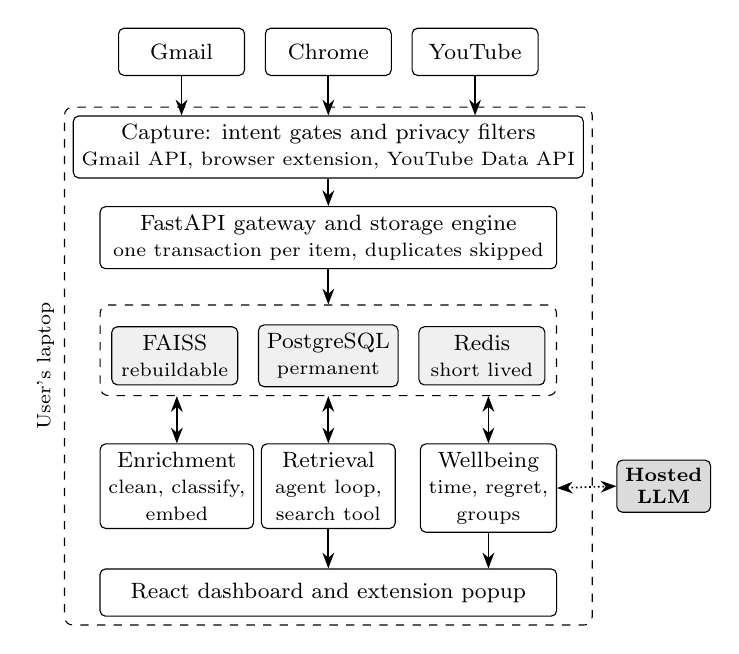
\begin{tikzpicture}[node distance=3.5mm and 2.5mm]
  \node[box, minimum width=16mm] (gm) {Gmail};
  \node[box, minimum width=16mm, right=of gm] (ch) {Chrome};
  \node[box, minimum width=16mm, right=of ch] (yt) {YouTube};
  \node[box, minimum width=58mm, below=5mm of ch] (cap)
      {Capture: intent gates and privacy filters\\ \scriptsize Gmail API, browser extension, YouTube Data API};
  \node[box, minimum width=58mm, below=of cap] (gw)
      {FastAPI gateway and storage engine\\ \scriptsize one transaction per item, duplicates skipped};
  \node[store, minimum width=16mm, below=7mm of gw] (pg) {PostgreSQL\\ \scriptsize permanent};
  \node[store, minimum width=16mm, left=of pg] (fa) {FAISS\\ \scriptsize rebuildable};
  \node[store, minimum width=16mm, right=of pg] (rd) {Redis\\ \scriptsize short lived};
  \node[grp, fit=(fa)(pg)(rd), inner ysep=5pt, yshift=2pt] (st) {};
  \node[box, minimum width=17mm, below=6mm of st.south west, anchor=north west] (enp)
      {Enrichment\\ \scriptsize clean, classify,\\ \scriptsize embed};
  \node[box, minimum width=17mm, below=6mm of st.south, anchor=north] (rse)
      {Retrieval\\ \scriptsize agent loop,\\ \scriptsize search tool};
  \node[box, minimum width=17mm, below=6mm of st.south east, anchor=north east] (wba)
      {Wellbeing\\ \scriptsize time, regret,\\ \scriptsize groups};
  \node[box, minimum width=58mm, below=5mm of rse] (ui) {React dashboard and extension popup};
  \node[grp, fit=(cap)(gw)(st)(enp)(wba)(ui), inner sep=3pt] (lap) {};
  \node[font=\scriptsize, rotate=90, anchor=south] at (lap.west) {User's laptop};
  \node[llm, minimum width=11mm, right=3mm of lap.east |- rse.east, anchor=west, font=\scriptsize\bfseries] (lm) {Hosted\\LLM};
  \draw[arr] (gm) -- (gm |- cap.north);
  \draw[arr] (ch) -- (cap);
  \draw[arr] (yt) -- (yt |- cap.north);
  \draw[arr] (cap) -- (gw);
  \draw[arr] (gw) -- (st.north);
  \draw[arr, {Stealth[length=2mm]}-{Stealth[length=2mm]}] (enp.north) -- (enp.north |- st.south);
  \draw[arr, {Stealth[length=2mm]}-{Stealth[length=2mm]}] (rse.north) -- (rse.north |- st.south);
  \draw[arr, {Stealth[length=2mm]}-{Stealth[length=2mm]}] (wba.north) -- (wba.north |- st.south);
  \draw[arr] (rse) -- (ui);
  \draw[arr] (wba.south) -- (wba.south |- ui.north);
  \draw[arr, densely dotted, {Stealth[length=2mm]}-{Stealth[length=2mm]}] (wba.east) -- (lm.west);
\end{tikzpicture}
\caption{Main parts of E.C.H.O. Everything inside the dashed frame runs on the user's laptop. The dotted arrow is the only path to the hosted language model; it carries short text from three callers (classification, retrieval, weekly reflection), described in Section~\ref{sec:privacy}.}
\label{fig:arch}
\end{figure}

% ---------------------------------------------------------------------
\section{Methodology}\label{sec:method}
% ---------------------------------------------------------------------
\subsection{Intent Aware Capture}
Each source has its own rule for what to keep, summarized in Table~\ref{tab:gates}. The values are the ones chosen for the final system; the browser and the server hold matching copies, so a page the extension sends is never silently refused by the server.

Gmail is treated differently from the other two sources. Mail arrives on its own rather than being chosen, daily volume is small, and even an unread message may matter later, so every message is stored when it arrives. The connector polls every 30 seconds, but each poll asks Gmail only for the changes since a saved history position instead of listing the whole mailbox. If that position has expired, the connector lists the mailbox once and the uniqueness rule on stored items absorbs the overlap. Mail that Gmail has filed as spam or trash is never read; Gmail's own spam filter acts as E.C.H.O's spam filter. When the user opens a message in Gmail on the web, the extension reports the message id and the seconds spent reading, and nothing else.

Chrome pages pass a two phase gate. In phase one the page must stay in the foreground for at least five seconds; a page that fails is dropped, and only a page that passes is remembered for revisit detection. In phase two at least one sign of attention must appear: enough foreground time, enough scrolling, a real interaction, or a visit to the same page within the last 24 hours. Selecting text or clicking inside the page counts as an interaction, but clicking a link does not, because a click that leaves the page shows a choice to go elsewhere rather than interest in the page itself. Time is counted only while the tab is active, the window has focus, and the user has not been idle for 30 seconds. Along with the text of the main content, the extension sends the page's top level headings, which later help the page be found by topic.

YouTube videos are kept when the user watches long enough, watches a large enough share of the video, pauses, seeks, or changes the speed, or returns to the same video within a day. The completion rule requires at least five seconds of real watching, so swiping past a short clip does not count as watching ten percent of it. After five seconds of watching, the extension records the visit, which lets a second short visit pass through the revisit rule. Shorts are recognized from the page address and have a lower time bar.

\begin{table}[t]
\caption{Capture Rules for Each Source}
\label{tab:gates}
\centering
\renewcommand{\arraystretch}{1.15}
\begin{tabular}{|>{\raggedright\arraybackslash}p{1.35cm}|>{\raggedright\arraybackslash}p{6.2cm}|}
\hline
\textbf{Source} & \textbf{An item is kept when} \\
\hline
Gmail & Always, at arrival, except mail in Spam or Trash. Polled every 30~s for changes only. Reading time is added when a message is opened (opens under 3~s are ignored). \\
\hline
Chrome & Phase 1: at least 5~s in the foreground. Phase 2: any one of at least 10~s in the foreground, at least 15\% scroll depth, one interaction other than a link click, or a revisit within 24~hours. Work app pages: at least 5~s or one interaction, title only. \\
\hline
YouTube & Any one of at least 20~s of foreground playback (10~s for Shorts), at least 10\% of the video watched with at least 5~s of watching, a pause, seek, or speed change by the user, or a revisit within 24~hours. \\
\hline
\end{tabular}
\end{table}

\subsection{Storage Model}
Each email, page, and video becomes one row in a central table of memory items. Fields that belong to one source go into a matching table for Gmail, Chrome, or YouTube, and attachments get a table of their own. Engagement counters such as reading time, watch time, and revisits live apart because they change often. Chrome and YouTube also write one row per admitted visit, with the time of the visit and the seconds spent, so that a page read on two different days is counted on both. The schema has 17 tables.
% 17 = the 16 tables in scripts/setup_db.py + the visit table (A1.1).
% Other decided schema changes: gmail_attachments.extracted_text (A4),
% stored tsvector + GIN index (A24.3), classification_confidence dropped
% (A21). A43 (still open) may add user_groups.system_group_id.

A uniqueness rule on the pair of source type and source id stops the same item from being stored twice, for example after a connector restart. Every item always carries one of the five system groups, with misc as the fallback. Items are first written in a raw state and flagged as unprocessed, which keeps the capture path short and safe against crashes. When a revisited page comes back with different text, it is flagged again so that its vector is rebuilt. Timestamps are stored in UTC and shown to the user in local time.

A user can delete a single item, which hides it from every query. Separately, a retention setting offers three choices: keep forever, keep one year, or keep six months. Keep forever is the default, because recalling old things is the point of the system. With a shorter window, a job at backend startup permanently removes older items from PostgreSQL, the FAISS index, and Redis together.

\subsection{Background Enrichment}
A background worker picks up unprocessed items every few seconds. It never runs on the capture path, so slow enrichment cannot slow capture. Each item goes through four steps.

\textit{Cleaning.} For email, HTML is converted to text with line breaks kept, and scripts, styles, tracking pixels, and hidden preview text are removed. A body that the sending app split around an inline image is joined back together. Quoted earlier messages are removed, but lines the sender typed between quoted lines are kept, since an inline reply is often the whole point of the message. Signatures are deliberately left in place: a heuristic remover we tested cut real body text in six of eight sample messages, while a leftover signature only adds a little noise. For a reply, keywords from earlier messages in the same thread are added, so a terse ``Re:'' can still be found by its topic. For web pages, the extension has already picked the main content and the headings; the worker separates the headings from the body. For videos, the text is the title, the channel, the category, the tags, the description, and the transcript. The server fetches the transcript with a transcript library, trying English captions first and automatic captions second; a video without captions is embedded without one.
% TODO A11: transcript source decided Thu 22 Oct (youtube-transcript-api,
% else no transcripts). If it fails, change the sentence above to
% "title, channel, category, tags, and description".

\textit{Attachments.} Attachment text is extracted in the same worker when the mail is processed. Supported types are PDF, DOCX, XLSX, PPTX, plain text formats such as TXT, CSV, Markdown, JSON, and calendar files, HTML, and forwarded messages. Images and scanned PDFs are read with Tesseract OCR \cite{b15}. Inline images such as signature logos and very small images are skipped. The extracted text is stored next to the attachment record, not inside the email body. The beginning of each attachment joins the email's embedded text, and the full text joins the keyword index, so content deep inside a file can still be found by keyword.

\textit{Embedding.} The cleaned text is turned into a \embdim{} dimension vector with the \embmodel{} sentence model \tbd{confirm final model, decision A40}. The text is assembled so that short hints come first: subject, keywords, and sender for mail; domain and headings for pages; channel and category for videos. Long text such as a body or a description comes last, so any trimming to the model's input window removes only the end of the long part \tbd{token budget, decision A16}. The vector is added to the FAISS index without rebuilding it.

\textit{Classification.} Every item receives one of five broad groups: work, study, entertainment, personal, or misc, through a four stage cascade. Stage one reads structural signals from the source, such as Gmail category labels, academic mail domains, or the YouTube video category. Stage two looks the web domain up in a curated table. Stage three compares the item's vector with a center point per group and accepts only a clear winner. Each center starts as the mean of several example sentences written for its group, and uses a lower acceptance bar while it is still a seed \tbd{seed threshold, measured on labeled rows}. Once a group has at least ten confirmed items, its center is recomputed from real items, with each source weighted equally so that a center learns a topic rather than the look of one source. A recomputed center accepts an item only if the cosine similarity is at least 0.55 and leads the second best group by at least 0.08. The recomputation runs when the worker starts, if the stored centers are missing or older than 30 days. Stage four asks the language model, one item at a time, using only the title and about 300 characters of text. With an OpenAI model the call is a typed choice among the five group names; with other providers the reply must be exactly one group name, and any other reply becomes misc. If the typed call raises an error, that item takes the single word path instead, so classification never stops. No confidence value is stored.

\textit{State tracking.} Each item ends as processed or failed. Failed items are kept apart and retried automatically, so a failure is never counted as done and never lost.
% Beyond build (carried over from Draft 1): today retry is manual via the
% ENP_RETRY_FAILED setting; no decision schedules automatic retry yet.

\subsection{Retrieval Loop}
Questions are answered by the loop in Fig.~\ref{fig:graph}. The language model, \llmname{}, receives the conversation so far, today's date, the question, and one tool called \texttt{search\_memories}. The tool takes a query, an optional list of sources, an optional time phrase, and an optional sender or domain. The model decides how to phrase the search and may issue several searches in parallel in one round, for instance one per source. After reading the results it either answers or searches again. A usual question needs one call that searches and one call that answers. The code allows at most five search rounds; after the fifth, the next call is made without the tool, which forces an answer. A question therefore costs between two and six model calls, and the bound is enforced by the program, not by the prompt.

\begin{figure}[t]
\centering
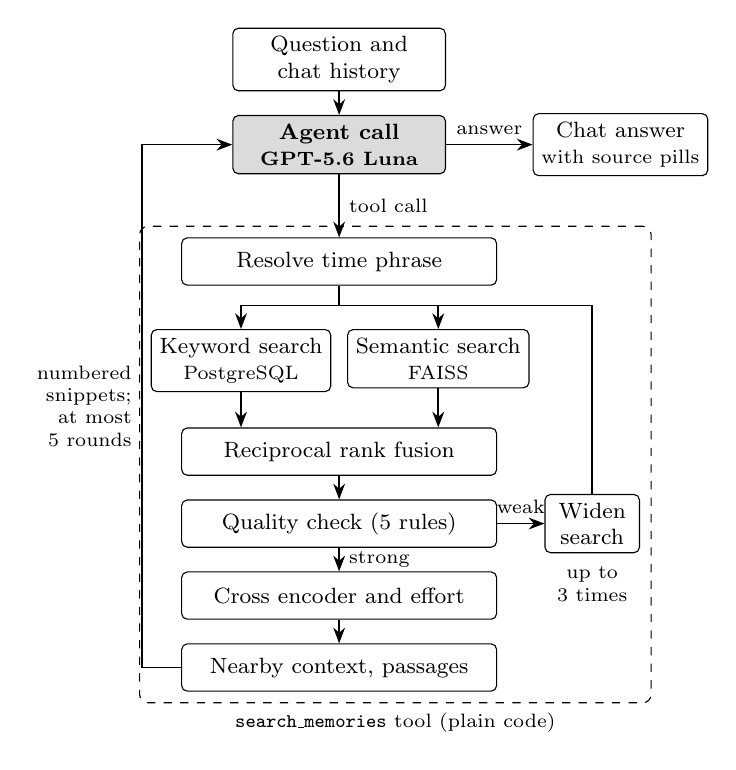
\begin{tikzpicture}[node distance=3mm and 3mm]
  \node[box, minimum width=27mm] (q) {Question and\\ chat history};
  \node[llm, minimum width=27mm, below=of q] (ag) {Agent call\\ \scriptsize\llmname};
  \node[box, minimum width=22mm, right=11mm of ag] (an) {Chat answer\\ \scriptsize with source pills};
  \node[box, minimum width=40mm, below=8mm of ag] (ta) {Resolve time phrase};
  \coordinate (bus) at ($(ta.south)+(0,-2.5mm)$);
  \node[box, minimum width=19mm, anchor=north east] (kw) at ($(bus)+(-1mm,-3mm)$) {Keyword search\\ \scriptsize PostgreSQL};
  \node[box, minimum width=19mm, anchor=north west] (se) at ($(bus)+(1mm,-3mm)$) {Semantic search\\ \scriptsize FAISS};
  \node[box, minimum width=40mm, anchor=north] (rrf) at ($(bus)+(0,-15.5mm)$) {Reciprocal rank fusion};
  \node[box, minimum width=40mm, below=of rrf] (qc) {Quality check (5 rules)};
  \node[box, minimum width=12mm, right=6mm of qc] (wd) {Widen\\search};
  \node[box, minimum width=40mm, below=of qc] (ce) {Cross encoder and effort};
  \node[box, minimum width=40mm, below=of ce] (nb) {Nearby context, passages};
  \node[grp, fit=(ta)(kw)(se)(rrf)(qc)(wd)(ce)(nb), inner sep=4pt] (tool) {};
  \node[font=\scriptsize, anchor=north] at (tool.south) {\texttt{search\_memories} tool (plain code)};
  \draw[arr] (q) -- (ag);
  \draw[arr] (ag) -- node[above, font=\scriptsize] {answer} (an);
  \draw[arr] (ag) -- node[right, font=\scriptsize] {tool call} (ta);
  \draw[semithick] (ta.south) -- (bus);
  \draw[semithick] (bus -| kw.center) -- (bus -| wd.center);
  \draw[arr] (bus -| kw.center) -- (kw.north);
  \draw[arr] (bus -| se.center) -- (se.north);
  \draw[semithick] (wd.north) -- (wd.north |- bus);
  \node[font=\scriptsize, align=center, below=0.5mm of wd] {up to\\3 times};
  \draw[arr] (kw.south) -- (kw.south |- rrf.north);
  \draw[arr] (se.south) -- (se.south |- rrf.north);
  \draw[arr] (rrf) -- (qc);
  \draw[arr] (qc) -- node[above, font=\scriptsize] {weak} (wd);
  \draw[arr] (qc) -- node[right, font=\scriptsize] {strong} (ce);
  \draw[arr] (ce) -- (nb);
  \draw[arr] (nb.west) -- ++(-5mm,0) |- node[pos=0.25, left, font=\scriptsize, align=right] {numbered\\snippets;\\at most\\5 rounds} (ag.west);
\end{tikzpicture}
\caption{The retrieval loop. The shaded box is the only place a language model is called. Everything inside the dashed frame is deterministic code with two small local encoders. When the search is widened, both search branches run again.}
\label{fig:graph}
\end{figure}

\textit{Resolve time phrase.} The model passes time words as written, and code turns them into dates. A calendar phrase such as ``last Tuesday'' becomes a start date. A phrase that points at another item, such as ``after the interview email,'' is looked up among the user's own items, first by keyword and then by meaning with a minimum similarity, and the time of the matching item becomes a hard limit for both search branches. If no anchor item is found, the search runs without that limit. Mail is matched by when it arrived, while pages and videos match when any recorded visit falls in the range. The date filter is open ended, so the answering call is told today's date and asked to use only items inside the period the user named.

\textit{Parallel search.} The keyword branch runs PostgreSQL full text search over a stored text index that covers titles, the full item text, attachment text, senders, domains, and channel names. The semantic branch embeds the query and searches FAISS. The two branches run in the same step of the graph.

\textit{Fusion.} The two ranked lists are merged with reciprocal rank fusion \cite{b9}. For an item $d$, the fused score is
\begin{equation}
\mathrm{RRF}(d) = \sum_{b \in B} \frac{1}{k + r_b(d)}, \label{eq:rrf}
\end{equation}
where $B$ is the set of branches that returned $d$, $r_b(d)$ is its position in branch $b$ starting from 1, and $k = 60$. Only positions are used, so the two score scales never need to be matched. The top 50 fused items move on.

\textit{Quality check and widening.} Five rules judge the fused list. It is weak or empty if it has no items, if no item comes from a source the user asked for, if no item falls inside the time window, if it holds fewer than two items, or if the best cosine similarity is below 0.35. A weak list triggers a wider search, and both branches run again. Each attempt relaxes more: the first stretches the time window by four days, opens all sources, or shortens the query to its core keyword; the second drops the time filter and the anchor; the third drops the keyword filters and searches a larger part of the vector index. After three attempts the tool reports that nothing was found, and the model can say so or try a different phrasing.
% 0.35 (rse/config.py MIN_TOP_SIMILARITY) was tuned on MiniLM. A39 says
% re-measure it on Thursday's data with the A40 model.

\textit{Reranking.} The local cross encoder \rerankmodel{} \cite{b10}, \cite{b11} scores each remaining item against the question. The final score blends this with an effort score:
\begin{equation}
s(d) = 0.8\,\sigma\big(c(q,d)\big) + 0.2\,e(d), \label{eq:final}
\end{equation}
where $c(q,d)$ is the cross encoder output for question $q$ and item $d$, $\sigma$ is the sigmoid function, and $e(d) \in [0,1]$ is the effort score. Effort is the mean of the engagement signals an item has, such as reading or watch time, scroll depth, revisits, interactions, and the share of a video watched, each capped and scaled to $[0,1]$. It favors items the user gave real attention to. Email is a special case: mail read on a phone, or never opened in the browser, has no measurable reading time. Instead of scoring such mail as zero, the reranker gives it the median effort of the other emails in the same result list, so an unmeasured email is neither punished nor promoted. By design, the score has no term for how recent an item is, and no diversity reranking is applied.

\textit{Nearby context and passages.} For the top three items, the tool adds close neighbors: other emails in the same thread, or pages and videos from the same browsing session or within five minutes. Each result reaches the model as a numbered entry with its title, source, time, the sender, site, or channel, and a 500 character window of its cleaned text. The window is the part that best matches the question, not simply the first 500 characters. When a result is an email with attachments and the question concerns their content, the three paragraphs of the stored attachment text that best match the question are added, about 1,500 characters in total. Numbers stay stable across rounds, so a citation always points to the same item.
% TODO A26 build: the live Gmail check (fetch_api node, "mail that just
% arrived") has no decided place in the tool loop yet; with 30 s
% incremental polling it may be dropped. Not described in the paper.

\textit{Writing the answer.} The final call writes a conversational reply in Markdown that leads with the direct answer, admits gaps plainly, and asks back in one line when the question is ambiguous. After each fact it places a hidden marker naming the numbered item that supports it. The backend keeps only markers that point to items the tool actually returned, so the model cannot cite a source it never saw. The dashboard turns each marker into a small pill that names the human anchor of the memory, such as the sender, the site, or the channel, plus a short date; clicking a pill opens the original email, page, or video. A thin time strip under the reply places each cited item on a timeline. While the loop runs, the dashboard streams progress messages such as which source is being searched, and then streams the reply itself.

\textit{Failure handling.} If the model cannot be reached, the deterministic pipeline runs once on the raw question and the user receives the ranked list of matching items instead of an error.

\subsection{Conversation Memory}
Each chat has a session id, and every turn is saved in PostgreSQL on the laptop. Opening an old chat resumes its session, so a follow up such as ``show me Chrome pages about that topic after that email'' can refer back to an earlier answer. Chat history older than 30 days is removed at startup.
% TODO A26: chaining turns with previous_response_id needs store=true at
% OpenAI, which still needs the owner's OK (doc 10.7 says history never
% goes to a cloud service). Not claimed here.

% ---------------------------------------------------------------------
\section{Wellbeing and User Groups}\label{sec:wba}
% ---------------------------------------------------------------------
The wellbeing module answers one question: where did my time go? Its rule is to describe, never to judge. It shows numbers and patterns and leaves the verdict to the user.

\textit{Time.} Time totals are computed on demand from the stored records and never stored separately, which avoids counting the same minutes twice. Page and video time come from the per visit rows, so each day receives exactly the time spent on that day. Email time comes from the reading time the extension reports. All days are the user's local days.

\textit{Sessions.} A session is a run of activity in which consecutive items are less than 20 minutes apart. The architecture first proposed five minutes, but each item is recorded at one point in time, so a 15 minute read followed by the next page looked like a 15 minute gap and split one sitting in two. For each session the module records its length, the system group with the most time, and how often the user switched between sources.

\textit{Regret.} Only the user decides what is regrettable. Any item can be marked, and every mark or unmark is stored as a new event, so the record is never overwritten and an item is currently regretted when its count of events is odd. The module reports how many marked items fall in each content type and hour, and flags a habit when the same kind of item at a similar hour is marked at least three times in 30 days.

\textit{Weekly reflection.} Once a week the module can write a short reflection. One language model call receives only aggregated numbers: totals per category, regret counts, session patterns, and peak hours. It never receives a title, an address, or any text from an item. The reply is checked for judging phrases before it is shown; if it fails the check or the call fails, a plain summary built from the same numbers is shown instead.

\textit{User groups.} System groups answer ``what kind of item is this?'' User groups answer ``which of my goals does it serve?'', for example ``Placement prep.'' A user group starts with items the user files by hand. Once it has five confirmed items, an assignment job scores other items against it in two ways: rules the user wrote (a keyword, domain, channel, sender, or date range) and a nearest neighbor score, the mean cosine similarity between the item and the three most similar confirmed members. An item is suggested when a rule matches, or when the neighbor score alone reaches a threshold \tbd{KNN only threshold, decision A32, set with the final model}. The module can also propose a new rule when at least five confirmed members share a domain, sender, or channel.

Every suggestion waits for the user. The only way an item enters a user group is an explicit accept in the review screen, and manual filing passes through the same recorded path, so each membership has an audit trail. A rejected suggestion is never offered again for that group. User groups are independent of the five system groups, so one goal can hold study pages and work mail together.
% TODO A42: auto accept of confident suggestions is still open. If decided,
% describe which score auto accepts and the weekly undo.
% TODO A43: user groups as children of system groups is still open. If
% decided, replace the last sentence above.

% ---------------------------------------------------------------------
\section{Privacy by Design}\label{sec:privacy}
% ---------------------------------------------------------------------
\textit{What is never captured.} Nothing from incognito windows is recorded, and neither is typed text or form input. A page whose address contains a sensitive word, matched as a whole word from a fixed list of 38 (for example login, password, checkout, otp, or netbanking), keeps no text. The same holds for a page with a visible password box or a form with several personal fields. Parameters that often carry secrets, such as tokens, one time codes, and session ids, are cut from every address before it is stored. Seven work apps (Slack, Atlassian, Notion, Figma, Linear, Trello, and Asana) are stored as page titles only, never as text, while their public help, blog, and documentation sections are treated as ordinary pages. Gmail on the web is skipped by browser capture, because mail already arrives through the Gmail API. The lists live in one copy on the server and the extension fetches them at startup; until they arrive, the extension extracts no text.

\textit{What leaves the laptop.} The database, the vector index, the cache, and both encoders run locally. Two kinds of traffic leave the machine. Requests to the Gmail and YouTube APIs fetch the user's own data. Calls to the hosted language model carry short text from three callers. Retrieval sends the question, the chat history, and numbered results, each a title, a time, a sender, site, or channel, and a 500 character excerpt, plus at most three short passages of attachment text when the user asks about a file. The classifier sends a title and about 300 characters, and only for items the first three stages could not place. The weekly reflection sends aggregated numbers only. Full emails, full pages, transcripts, database rows, and vectors are never sent.

\textit{Captured text is data, not instructions.} A stored email or page might contain text written to steer a language model. The search tool is read only and the system prompt tells the model that every snippet is data, which limits what such text can achieve. Retrieval logs record counts, scores, and timings, not questions or titles.

\textit{User control.} Each source can be switched off, domains and senders can be excluded, and capture can be paused from the extension popup. Items can be deleted, all data can be exported as JSON or CSV, and the retention setting removes old data for good.

% ---------------------------------------------------------------------
\section{Implementation}\label{sec:impl}
% ---------------------------------------------------------------------
Table~\ref{tab:stack} lists the technology. The backend is Python served by FastAPI. The retrieval loop is a LangGraph graph \cite{b5} in which an agent node and a tool node alternate under a round counter. Every model call goes through LangChain, so a different provider is a change to one configuration entry. When the provider is OpenAI, the code also turns on provider specific features: the Responses API, a medium reasoning effort for both retrieval calls, and the typed choice used by the classifier. Embeddings and the cross encoder run locally on the CPU through the sentence transformers library. The dashboard is React with TypeScript, and the extension uses Chrome Manifest V3.

PostgreSQL 16 runs as a native service on the laptop, and Redis runs locally under the Windows Subsystem for Linux. Development used hosted database and cache services; the final system moved both to the laptop, which also means that only standard HTTPS traffic leaves the machine.

\begin{table}[t]
\caption{Technology Used in the Final System}
\label{tab:stack}
\centering
\renewcommand{\arraystretch}{1.15}
\begin{tabular}{|>{\raggedright\arraybackslash}p{2.0cm}|>{\raggedright\arraybackslash}p{5.55cm}|}
\hline
\textbf{Layer} & \textbf{Technology} \\
\hline
Capture & Chrome extension (Manifest V3), Gmail API, YouTube Data API \\
\hline
Backend & Python, FastAPI, server sent events \\
\hline
Storage & PostgreSQL 16, FAISS, Redis, all local \\
\hline
Enrichment & Text extraction for PDF, DOCX, XLSX, PPTX, and EML; Tesseract OCR \\
\hline
Models & \embmodel{} embeddings, \rerankmodel{} cross encoder, \llmname{} through the OpenAI Responses API \\
\hline
Retrieval & LangGraph, LangChain \\
\hline
Interface & React, TypeScript, Vite \\
\hline
\end{tabular}
\end{table}

% ---------------------------------------------------------------------
\section{Evaluation Protocol}\label{sec:eval}
% ---------------------------------------------------------------------
This draft reports no measured results. Every value below marked TBD will be filled in from measurements on the final build.

\subsection{Data and Questions}
The evaluation uses the project's test account, restored into the local database: \tbd{number of items per source}. The team will write \tbd{number of questions} questions with known relevant items. They cover five kinds of need: a single source, several sources, a time anchored question (``after the interview email''), a follow up that refers to an earlier turn, and a question about attachment content.

\subsection{Retrieval Quality}
We compare four configurations: keyword search alone, semantic search alone, fusion without the cross encoder, and the full pipeline. We report Recall@10 and the mean reciprocal rank of the first relevant item (Table~\ref{tab:results}). The same question set is also run through the full agent loop to see whether letting the model rephrase and repeat searches finds items the single pass misses.

\begin{table}[t]
\caption{Retrieval Quality (to be measured)}
\label{tab:results}
\centering
\renewcommand{\arraystretch}{1.15}
\begin{tabular}{|l|c|c|}
\hline
\textbf{Configuration} & \textbf{Recall@10} & \textbf{MRR} \\
\hline
Keyword only & \textbf{[TBD]} & \textbf{[TBD]} \\
\hline
Semantic only & \textbf{[TBD]} & \textbf{[TBD]} \\
\hline
Fusion, no cross encoder & \textbf{[TBD]} & \textbf{[TBD]} \\
\hline
Full pipeline & \textbf{[TBD]} & \textbf{[TBD]} \\
\hline
Full agent loop & \textbf{[TBD]} & \textbf{[TBD]} \\
\hline
\end{tabular}
\end{table}

\subsection{Cost and Speed}
For each question we log the number of model calls, the number of search rounds, input and output tokens, and the end to end time on the team's laptop. We will report the mean number of calls \tbd{mean LLM calls per question} and how often the five round cap was reached \tbd{share of questions hitting the cap}, the median and 95th percentile response time \tbd{latency, seconds}, and the cost per question \tbd{cost per question}.

\subsection{Capture Accuracy}
Scripted browsing and viewing sessions (a page closed after two seconds, a page scrolled but left quickly, a Short swiped past, a tutorial watched halfway) are replayed, and the stored items are compared with what each rule should keep \tbd{agreement of the gates with the scripted labels}.

\subsection{Privacy Audit}
Every request to the language model is logged during the evaluation. We check that no request contains a full email, page, or transcript, and report the largest request seen \tbd{largest request, characters}.

\subsection{Threshold Calibration}
Three similarity cutoffs depend on the embedding model and will be set on the restored data once the model is fixed: the seed acceptance bar of classification stage three, the nearest neighbor bar for group suggestions, and the 0.35 floor of the quality check. For the first two, we pick the lowest value that produces no wrong assignment on items with known labels.

% ---------------------------------------------------------------------
\section{Limitations and Future Work}\label{sec:limits}
% ---------------------------------------------------------------------
E.C.H.O has clear limits. It targets desktop Chrome, so phone activity is invisible. YouTube history starts the day the extension is installed, and background or picture in picture playback is not tracked. One vector per item means that only the beginning of a long document shapes its meaning based match; deep content is reachable by keyword only. Replies from Outlook quote the older thread without a marker E.C.H.O removes, so such threads can appear more than once in results. The date filter is open ended, and only the top ten results reach the answering call, so on a busy day a question about yesterday could be crowded out by today's items. Pages of private apps outside the seven listed, such as chat assistants or online documents, are captured as ordinary pages unless the user excludes their domain. The OAuth tokens are kept as plain files on the laptop and are protected only by the operating system's file permissions. Finally, the language model is a hosted service, so its availability and limits apply.

Future work starts with the evaluation in Section~\ref{sec:eval}. Beyond it, we plan to store several vectors per long item, to let the domain table learn from the user's own confirmed labels, to accept very confident group suggestions automatically while keeping them open to a weekly undo, and to optionally nest user groups under system groups. Importing past history from Google Takeout and the browser's own history file would let a new user start with a full memory instead of an empty one. Exposing the search tool through the Model Context Protocol would let other assistants query the same memory under the same privacy rules.
% A42 / A43 / E1 / E2 are listed above as future work only. Update this
% paragraph if A42 or A43 is decided before submission.

% ---------------------------------------------------------------------
\section{Conclusion}\label{sec:conc}
% ---------------------------------------------------------------------
E.C.H.O turns email, browsing, and video history into one personal memory that can be searched in plain language. It keeps all legitimate mail but only the pages and videos the user paid attention to, stores them on the user's laptop, and prepares them for search in the background. Questions are answered by a loop in which a language model plans the search and deterministic code performs it, so the model's role is visible, bounded, and cheap. Around it, a wellbeing module describes how time is spent and keeps the user in charge of every personal grouping. The next version of this paper will report the measurements laid out above.

\section*{Acknowledgment}
We thank the Department of Computer Science and Engineering, PES University, for its support during this capstone project.

% Balances the two columns on the last page. Adjust the number if the reference list changes.
\IEEEtriggeratref{10}
\begin{thebibliography}{00}
\bibitem{b1} V. Bush, ``As we may think,'' \textit{The Atlantic Monthly}, vol. 176, no. 1, pp. 101--108, Jul. 1945.
\bibitem{b2} S. Dumais, E. Cutrell, J. J. Cadiz, G. Jancke, R. Sarin, and D. C. Robbins, ``Stuff I've seen: A system for personal information retrieval and re-use,'' in \textit{Proc. 26th Annu. Int. ACM SIGIR Conf. Research and Development in Information Retrieval}, Toronto, Canada, 2003, pp. 72--79.
\bibitem{b3} J. Gemmell, G. Bell, and R. Lueder, ``MyLifeBits: A personal database for everything,'' \textit{Commun. ACM}, vol. 49, no. 1, pp. 88--95, Jan. 2006.
\bibitem{b4} P. Lewis, E. Perez, A. Piktus, F. Petroni, V. Karpukhin, N. Goyal, H. K\"{u}ttler, M. Lewis, W. Yih, T. Rockt\"{a}schel, S. Riedel, and D. Kiela, ``Retrieval-augmented generation for knowledge-intensive NLP tasks,'' in \textit{Advances in Neural Information Processing Systems}, vol. 33, 2020, pp. 9459--9474.
\bibitem{b5} LangChain, ``LangGraph,'' GitHub repository. [Online]. Available: \url{https://github.com/langchain-ai/langgraph} (accessed Oct. 21, 2026).
% b13 verified 2026-10-21 (arXiv 2210.03629, ICLR 2023 proceedings listing).
\bibitem{b13} S. Yao, J. Zhao, D. Yu, N. Du, I. Shafran, K. Narasimhan, and Y. Cao, ``ReAct: Synergizing reasoning and acting in language models,'' in \textit{Proc. 11th Int. Conf. Learning Representations (ICLR)}, Kigali, Rwanda, 2023.
\bibitem{b6} N. Reimers and I. Gurevych, ``Sentence-BERT: Sentence embeddings using Siamese BERT-networks,'' in \textit{Proc. 2019 Conf. Empirical Methods in Natural Language Processing and 9th Int. Joint Conf. Natural Language Processing (EMNLP-IJCNLP)}, Hong Kong, China, 2019, pp. 3982--3992.
\bibitem{b8} J. Johnson, M. Douze, and H. J\'{e}gou, ``Billion-scale similarity search with GPUs,'' \textit{IEEE Trans. Big Data}, vol. 7, no. 3, pp. 535--547, Jul. 2021.
\bibitem{b9} G. V. Cormack, C. L. A. Clarke, and S. B\"{u}ttcher, ``Reciprocal rank fusion outperforms Condorcet and individual rank learning methods,'' in \textit{Proc. 32nd Int. ACM SIGIR Conf. Research and Development in Information Retrieval}, Boston, MA, USA, 2009, pp. 758--759.
\bibitem{b10} R. Nogueira and K. Cho, ``Passage re-ranking with BERT,'' arXiv:1901.04085, 2019.
\bibitem{b7} W. Wang, F. Wei, L. Dong, H. Bao, N. Yang, and M. Zhou, ``MiniLM: Deep self-attention distillation for task-agnostic compression of pre-trained transformers,'' in \textit{Advances in Neural Information Processing Systems}, vol. 33, 2020, pp. 5776--5788.
\bibitem{b11} P. Bajaj \textit{et al.}, ``MS MARCO: A human generated machine reading comprehension dataset,'' arXiv:1611.09268, 2016.
\bibitem{b12} M. Kleppmann, A. Wiggins, P. van Hardenberg, and M. McGranaghan, ``Local-first software: You own your data, in spite of the cloud,'' in \textit{Proc. ACM SIGPLAN Int. Symp. New Ideas, New Paradigms, and Reflections on Programming and Software (Onward!)}, 2019, pp. 154--178.
% b14: verified 2026-10-21 (arXiv 1902.00157; Oxford CS publication 12395): authors
% Lyngs, Lukoff, Slovak, Binns, Slack, Inzlicht, Van Kleek, Shadbolt; DOI below.
\bibitem{b14} U. Lyngs \textit{et al.}, ``Self-control in cyberspace: Applying dual systems theory to a review of digital self-control tools,'' in \textit{Proc. CHI Conf. Human Factors in Computing Systems (CHI '19)}, Glasgow, UK, 2019, doi: 10.1145/3290605.3300361.
% b15 verified 2026-10-21 (research.google publication page, IEEE Xplore 4376991).
\bibitem{b15} R. Smith, ``An overview of the Tesseract OCR engine,'' in \textit{Proc. 9th Int. Conf. Document Analysis and Recognition (ICDAR)}, Curitiba, Brazil, 2007, pp. 629--633.
\end{thebibliography}

\end{document}
